%!TeX root=MemoriaTFG.tex
\chapter{Disseny de la solució}\label{disseny}
En aquest capítol es veurà quina ha estat la sol·lució al problema analitzat a l'apartat anterior. Es tracta de desenvolupar una \ac{API} que permeti als integrant de la comunitat universitaria gaudir d'un servei de missatgeria. Aquesta \ac{API} ha de servir de suport a diferents clients (aplicacions d'escriptori, aplicacions mòbils o aplicacions web entre d'altres). \\

En primer lloc s'exposa una visió global de les parts de l'aplicació. A continuació es farà una explicació detallada de cada mòdul de l'aplicació. S'ha dividir l'aplicació en els següents mòduls: 
\begin{itemize}

	\item \textbf{Model de dades:} s'explicarà com s'ha estructurat el model de dades replicat.
	\item \textbf{Serveis:} s'explicarà l'arquitectura \ac{SOA}, com s'ha estructurat, els diferents serveis que s'han desenvolupat i llibreries per donar suport a aquests.
	\item \textbf{\ac{API}:} s'explicarà com s'ha estructurat l'\ac{API} que s'ha dissenyat. En aquest apartat també s'explicarà com s'han definit i implementat els nivells d'accés als recursos de l'\ac{API}.
	\item \textbf{Integració contínua:} s'explicarà com s'han elaborat els tests unitaris per comprovar el correcte funcionament de l'aplicació. També s'explicarà el funcionament del servei \textbf{Travis CI} per a assegurar que cada desplegament a producció no altera el correcte funcionament del servei.
	
\end{itemize}

Una descripció a alt nivell de l'estructura de l'aplicació sería la següent: quan es fà una petició a l'\ac{API}, aquesta crida a un determinat servei que de manera abstracta realitza operacions sobre les dades (lectura o escriptura) residents a la base de dades. Una vegada fetes les operacions sobre la base de dades, el resultat d'aquesta es serialitza i l'\ac{API} s'encarrega de mostrar les dades a l'usuari. Es pot veure aquesta estructura a la figura \ref{fig:estructura}.

\begin{figure}[h!]
    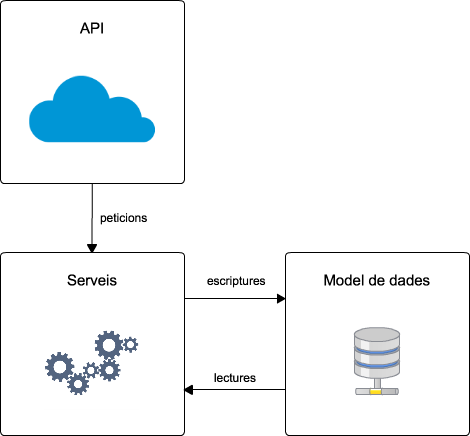
\includegraphics[scale=0.7]{img/estructura.png}
    \centering
    \caption{Visió global de com es connecten els tres principals mòduls de l'aplicació}
    \label{fig:estructura}
\end{figure}

\section{Model de dades}
Per preservar la independència de les dades del nostre sistema de les dades de la universitat, s'ha decidit replicar les dades necessàries al nostre sistema per no operar directament sobre el conjunt de dades de la universitat, per no dependre de la estructura que manté la universitat i per no alterar el rendiment dels sistemes de la universitat.\\

S'ha dissenyat una estructura de dades de manera que no depengui de cap universitat i pugui ser usada per qualsevol institució educativa. A la figura \ref{fig:model} es pot veure el model de dades resultant. \\

\begin{figure}[here]
    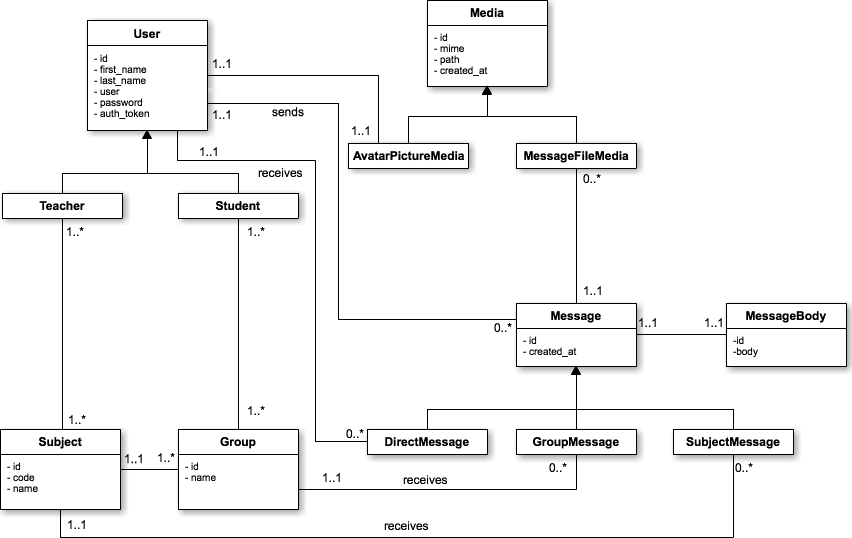
\includegraphics[scale=0.5]{img/uml.png}
    \centering
    \caption{Model de dades}
    \label{fig:model}
\end{figure}

Les entitats del model dissenyat són les següents: usuari, professor, estudiant, assignatura, grup, missatge, cos del missatge, missatge directe, missatge de grup, missatge d'assignatura, fitxer, avatar de l'usuari i fitxer de missatge. A continuació s'explicarà cada entitat del model.

	\subsection{Usuari, professor i estudiant} \label{user_teacher_student}

	L'entitat Usuari representa qualsevol usuari que interactuï amb l'\ac{API}. Un usuari està composat pels següents camps: 
	\begin{itemize}
		\item \textbf{id:} identificador únic de l'usuari. És un camp numèric i auto incremental.
		\item \textbf{first\_name:} nom de l'usuari.
		\item \textbf{last\_name:} cognoms de l'usuari.
		\item \textbf{user:} usuari d'accés al sistema. S'ha decidit per defecte s'intenti que aquest coincideixi amb les credencials d'accés a l'intranet de la universitat que implementi el servei.
		\item \textbf{password:} contrassenya d'accés al sistema. S'ha decidit que per defecte s'intenti que aquesta coincideixi amb la mateixa de les credencials d'accés a la intranet de la universitat que implementi el servei. 
		\item \textbf{auth\_token:} token d'autorització al sistema. S'explica amb més detall a la secció %TODO.
	\end{itemize}
	
	Com es veu al diagrama de classes del model de dades (figura \ref{fig:model}), les entitats Professor i Estudiant hereden de l'entitat Usuari. No hi ha cap diferència en els atributs de les entitats filles d'Usuari, a la pràctica s'ha afegit una variable de típus enter que diferencia si un usuari és professor, alumne i és ampliable a nous tipus (per exemple: un administrador, \ac{PAS}, etc...). \\
	
	Per implementar aquesta distinció entre professor i alumne, amb l'ajut de SQLAlchemy s'ha creat les entitats Usuari i TipusUsuari. L'entitat TipusUsuari representa els diferents típus d'usuari que hi pot haver, en el nostre cas  representarà o bé un professor o bé un alumne. Com es pot veure a la figura \ref{fig:entitats_usuari} l'entitat Usuari té una clau forana a TipusUsuari, d'aquesta manera relacionam l'usuari amb el seu tipus. \\
	
	Un altre aspecte a destacar de l'entitat Usuari és el token d'autorització al sistema. Aquest aspecte s'explicarà en l'apartat %TODO. 
	

\begin{figure}[here]
	\begin{python}
	class UserType:
	
    	TEACHER = 1
    	STUDENT = 2

    	id = Column(Integer, primary_key=True)
    	name = Column(String(15))
    	
	class User:
	
    	id = Column(BigInteger, primary_key=True)
    	first_name = Column(String(60))
    	last_name = Column(String(120))

    	user = Column(String(32), unique=True)
    	password = Column(String(256))
   		auth_token = Column(String(64))
    	type_id = Column(Integer, ForeignKey('user_type.id'))
    	type = relationship(UserType, backref=backref('users', uselist=True, cascade='delete,all'))
    	
    	def is_teacher(self):
    		return self.type.id == UserType.TEACHER
    		
    	def is_student(self):
    		return self.type.id == UserType.STUDENT
	\end{python}
    \caption{Entitats d'usuari, professor i alumne}
    \label{fig:entitats_usuari}
\end{figure}

	\subsection{Media, avatar i fitxer de missatge} \label{media_avatar_message}
	L'entitat Media representa el contingut multimèdia que un usuari pot publicar al servei. Es distingeix entre un avatar i un fitxer de missatge. Un avatar és la fotografia de perfil de l'usuari i un fitxer de missatge és un fitxer que pertany a un únic missatge. \\
	
	Una entitat Media està composada pels següents atributs:
	
	\begin{itemize}
		\item \textbf{id:} identificador únic de l'element multimèdia.
		\item \textbf{type:} tipus de multimèdia. S'explicarà a continuació.
		\item \textbf{mime:} típus \ac{MIME} del fitxer.
		\item \textbf{path:} ruta del fitxer físic al sistema de fitxers del servidor.
		\item \textbf{created\_at:} \emph{timestamp} de creació del fitxer.
	\end{itemize}
	
	En aquest cas, la diferència entre els dos típus de multimèdia és amb quina altra entitat del nostre sistema estàn relacionats. En el cas d'un avatar d'usuari aquest es relaciona amb l'usuari, en el cas d'un fitxer de missatge es relacionara amb un missatge.\\

	Una pregunta que es pot formular el lector és per què s'ha creat una entitat per l'avatar de l'usuari si aquest podria ser un atribut de l'entitat Usuari (veure seccio \ref{user_teacher_student}). La resposta a aquesta pregunta és per tenir la mateixa interfície d'accés als avatars d'usuari que als fitxers multimèdia. Ambdos típus de multimèdia es comportaràn de la mateixa manera i amb aquesta implementació tenim tot el contigut multimèdia centralitzat en una única entitat.	\\
	
	SQLAlchemy ens brinda la oportunitat de fer us de herència d'entitats. Per implementar-ho hem creat les següents entitats: Media, Avatar i FitxerDeMissatge. L'entitat Avatar té una clau forana cap a l'entitat Usuari (veure secció \ref{user_teacher_student}), mentre que l'entitat FitxerDeMissatge te la clau forana cap a l'entitat Missatge (veure secció \ref{message_direct_group_subject}). Es pot veure el codi de les tres entitats a la figura \ref{fig:entitats_multimedia}. \\
	

\begin{figure}[p]
	\begin{python}
class MediaType:
	
	AVATAR = 1
	MESSAGE_FILE = 2
		
	id = Column(Integer, primary_key=True)
	name = Column(String(20))
    	
class Media:

    id = Column(BigInteger, primary_key=True)
    type = Column(Integer, ForeignKey('media_type.id'))
    mime = Column(String(64))
    path = Column(String(256))
    created_at = Column(DateTime)

    __mapper_args__ = {'polymorphic_on': type}

class AvatarMedia(Media):
	
    user_id = Column(BigInteger, ForeignKey('user.id'), unique=True)
    user = relationship(User,  backref=backref('avatar', uselist=True, cascade='delete,all'))

    __mapper_args__ = {'polymorphic_identity': MediaType.AVATAR}

class MessageFileMedia(Media):

    message_id = Column(BigInteger, ForeignKey('message.id'))
    message = relationship(backref=backref('media', uselist=True, cascade='delete,all'))

    __mapper_args__ = {'polymorphic_identity': MediaType.MESSAGE_FILE}
    	
	\end{python}
    \caption{Entitats multimedia}
    \label{fig:entitats_multimedia}
\end{figure}
   
    Al igual que hem fet amb l'entitat Usuari, amb l'entitat Media també hem definit una entitat auxiliar: TipusMedia. Aquesta entitat auxiliar ens servirà per diferenciar entre els dos típus de contingut multimèdia que tenim. El seu comportament és el mateix que l'entitat TipusUsuari.\\
    
    Com que entre les dues entitats filles de Media hi ha diferència, en aquest cas s'ha optat per usar la herència que ens brinda la \ac{POO}. A nivell de llenguatge de programació s'ha fet que les classes Avatar i FitxerDeMissatge heretin de Media. A nivell de base de dades, s'ha d'indicar a l'\ac{ORM} quin camp de l'entitat pare ha d'usar per discriminar entre ambdos típus de multimèdia. És en aquest punt on entra en joc l'entitat TipusMedia. Si ens fixam en el codi de la figura \ref{fig:entitats_multimedia} podem veure com les dues entitats filles de Media tenen l'atribut \texttt{\_\_mapper\_args\_\_}. Aquest atribut defineix, entre d'altres, quin valor ha de tenir l'atribut \texttt{type} per que es pugui distingir una entitat de l'altra.\\
    
    Un altre aspecte a destacar del codi dels models són les relacions a les classes filles. Es pot observar que tant l'entitat Avatar i FitxerDeMissatge tenen dos atributs cada una. Per una banda Avatar te \texttt{user\_id} i \texttt{user}, per l'altra banda, l'entitat FitxerDeMissatge te \texttt{message\_id} i \texttt{message}. En ambdos casos, el primer es la clau forana cap a l'entitat que correspongui (Usuari en el cas d'Avatar i Missatge en el cas de FitxerDeMissatge). El segon atribut representa l'entitat a la qual fan referència. Si tenim una entitat Avatar amb \texttt{user\_id = 1}, el valor de \texttt{user} serà l'usuari amb \texttt{id = 1}.\\
   
    \subsection{Missatge, directe, de grup, d'assignatura i cos del missatge}\label{message_direct_group_subject}
    
    L'entitat Missatge representa qualsevol típus de missatge, ja sigui directe, a un grup o a una assignatura. A continuació es pot veure una relació dels atributs de l'entitat missatge:
    
    \begin{itemize}
    	\item \textbf{id:} identificador únic del missatge.
    	\item \textbf{type:} típus de missatge. El seu funcionament és el mateix que el típus multimèdia explicat a la secció \ref{media_avatar_message}.
    	\item \textbf{sender\_id:} identificador de l'usuari que envia el missatge. 
    	\item \textbf{body\_id:} identificador del cos del missatge. S'explicarà amb més detall a continuació.
    \end{itemize}
    
     Aquesta entitat també fa ús de l'herència que ens brinda la \ac{POO}. En aquest cas, hem de distingir tres típus de missatge: MissatgeDirecte, MissatgeGrup i MissatgeAssignatura. Tots tres típus de missatge tenen com a remitent un usuari, ja sigui professor o alumne. Un missatge directe va dirigit a un usuari, un missatge de grup va dirigit a un grup d'assignatura i un missatge d'assignatura va dirigit a una assignatura, al que anomenarem fòrum general de l'assignatura. \\
    
   	La implementació de l'herència és la mateixa que la que s'ha usat per l'entitat Media (veure secció \ref{media_avatar_message}) i no entrarem en detall en la seva implementació. També és fa us de la tècnica \texttt{relationship} que ens relaciona la clau forana amb l'entitat que correspon. \\
   	
   	L'entitat MissatgeDirecte conté una clau forana cap a usuari que referencia l'usuari al qual s'ha enviat el missatge. L'entitat MissatgeGrup conté una clau forana cap al grup que referencia el grup al qual s'ha enviat el missatge. L'entitat MissatgeAssignatura conté una clau forana cap a l'assignatura que referencia l'assignatura a la qual s'ha enviat el missatge.\\
   	
   	Per una altra banda, s'ha creat l'entitat CosDeMissatge que representa el contingut del missatge. S'ha definit una longitud màxima d'aquest de quatre-cents caràcters. Al ser el cos del missatge de longitud variable, cada registre tendrà un tamany variable i quedaràn espais de memòria reservats per el cos del missatge buits a disc. Per aquest motiu s'ha traslladat el contigut del missatge a una entitat apart i així l'entitat Missatge queda més compactada i fora espais de memoria buits.\\
   	
   	\subsection{Assignatura i grup}
   	
   	L'entitat Assignatura representa qualsevol assignatura que es pugui impartir dins la universitat. Una assignatura està composada pels següents atributs:
   	
   	\begin{itemize}
   		\item \textbf{id:} identificador únic de l'assignatura.
   		\item \textbf{code:} codi unic de l'assignatura, si escau.
   		\item \textbf{name:} nom de l'assignatura.
   	\end{itemize}
   	
   	L'entitat Grup representa qualsevol grup que pertanyi a una assignatura que es pugui impartir dins la universitat. Un grup està composat pels següents atributs:
   	
   	\begin{itemize}
   		\item \textbf{id:} identificador únic del grup.
   		\item \textbf{nom:} nom del grup.
   		\item \textbf{subject\_id:} identificador de l'assignatura que el grup pertany. 
   	\end{itemize}
   	
   	Segons el model de dades (veure figura \ref{fig:model}) un grup pertany només a una assignatura. Per aquest motiu l'entitat Grup conté una clau forana cap a l'entitat Assignatura.\\
   	
   	S'han creat dues entitats, ProfessorAssignatura i AlumneGrup. La primera fà referència a la relació entre professor i assignatura. En aquesta entitat es poden trobar els següents atributs:
   	
   	\begin{itemize}
   		\item \textbf{teacher\_id:} identificador del professor. A la pràctica fà referència a un identificador d'usuari.
   		\item \textbf{subject\_id:} identificador de l'assignatura.
   	\end{itemize}
   	
   	Ambdos atributs actúen com a clau primària de la taula, fet que implica que no faci falta tenir  un atribut \texttt{id} que actuï com a tal. El mateix fenòmen succeeix a l'entitat AlumneGrup, que té els següents atributs:
   	
   	\begin{itemize}
   		\item \textbf{student\_id:} identificador de l'alumne. A la pràctica fa referència a un identificador d'usuari.
   		\item \textbf{group\_id:} identificador del grup.
   	\end{itemize}
   	
   Al igual que amb l'entitat ProfessorAssignatura, ambdos atributs actúen com a clau primària,fet que implica que no faci falta tenir un atribut \texttt{id} que actuï com a tal.

\section{Serveis}

\section{\ac{API}}
	
\section{Integració contínua}


